\documentclass[nojss]{jss}\usepackage[]{graphicx}\usepackage[]{color}
%% maxwidth is the original width if it is less than linewidth
%% otherwise use linewidth (to make sure the graphics do not exceed the margin)
\makeatletter
\def\maxwidth{ %
  \ifdim\Gin@nat@width>\linewidth
    \linewidth
  \else
    \Gin@nat@width
  \fi
}
\makeatother

\definecolor{fgcolor}{rgb}{0.345, 0.345, 0.345}
\newcommand{\hlnum}[1]{\textcolor[rgb]{0.686,0.059,0.569}{#1}}%
\newcommand{\hlstr}[1]{\textcolor[rgb]{0.192,0.494,0.8}{#1}}%
\newcommand{\hlcom}[1]{\textcolor[rgb]{0.678,0.584,0.686}{\textit{#1}}}%
\newcommand{\hlopt}[1]{\textcolor[rgb]{0,0,0}{#1}}%
\newcommand{\hlstd}[1]{\textcolor[rgb]{0.345,0.345,0.345}{#1}}%
\newcommand{\hlkwa}[1]{\textcolor[rgb]{0.161,0.373,0.58}{\textbf{#1}}}%
\newcommand{\hlkwb}[1]{\textcolor[rgb]{0.69,0.353,0.396}{#1}}%
\newcommand{\hlkwc}[1]{\textcolor[rgb]{0.333,0.667,0.333}{#1}}%
\newcommand{\hlkwd}[1]{\textcolor[rgb]{0.737,0.353,0.396}{\textbf{#1}}}%

\usepackage{framed}
\makeatletter
\newenvironment{kframe}{%
 \def\at@end@of@kframe{}%
 \ifinner\ifhmode%
  \def\at@end@of@kframe{\end{minipage}}%
  \begin{minipage}{\columnwidth}%
 \fi\fi%
 \def\FrameCommand##1{\hskip\@totalleftmargin \hskip-\fboxsep
 \colorbox{shadecolor}{##1}\hskip-\fboxsep
     % There is no \\@totalrightmargin, so:
     \hskip-\linewidth \hskip-\@totalleftmargin \hskip\columnwidth}%
 \MakeFramed {\advance\hsize-\width
   \@totalleftmargin\z@ \linewidth\hsize
   \@setminipage}}%
 {\par\unskip\endMakeFramed%
 \at@end@of@kframe}
\makeatother

\definecolor{shadecolor}{rgb}{.97, .97, .97}
\definecolor{messagecolor}{rgb}{0, 0, 0}
\definecolor{warningcolor}{rgb}{1, 0, 1}
\definecolor{errorcolor}{rgb}{1, 0, 0}
\newenvironment{knitrout}{}{} % an empty environment to be redefined in TeX

\usepackage{alltt}
\usepackage{url}
\usepackage[sc]{mathpazo}
\usepackage{geometry}
\geometry{verbose,tmargin=2.5cm,bmargin=2.5cm,lmargin=2.5cm,rmargin=2.5cm}
\setcounter{secnumdepth}{2}
\setcounter{tocdepth}{2}
\usepackage{breakurl}
\usepackage{hyperref}
\usepackage[ruled, vlined]{algorithm2e}
\usepackage{mathtools}
\usepackage{draftwatermark}
\usepackage{float}
\usepackage{placeins}
%% \usepackage{mathbbm}
\DeclareMathOperator{\sgn}{sgn}
\DeclareMathOperator*{\argmax}{\arg\!\max}








\title{\bf Statistical Working Paper on Imputation and Validation
  Methodology for the FAOSTAT Production Domain}

\author{Michael C. J. Kao\\ Food and Agriculture Organization \\ of
  the United Nations}

\Plainauthor{Michael. C. J. Kao} 

\Plaintitle{Statistical Working Paper on Imputation and Validation
  Methodology for the FAOSTAT Production Domain}

\Shorttitle{Imputation and Validation Methodology}

\Abstract{ 

  This paper proposes a new imputation method for the FAOSTAT
  production domain based on linear mixed model and the EM-algorithm.
  The proposal provides resolve to many of the shortcomings of the
  current approach, and offers a flexible and robust framework to
  incorporate further information to improve performance.  
  
  We first examine the factors that drive changes in production by
  commodity, after which a brief acount of the current approach and
  its shortcomings. A description of the new methodology is provided.
  
  Finally, a case study on wheat is given with the fit, diagnostic and
  simulation results presented and closed with discussion.

}

\Keywords{Imputation, Linear Mixed Model, Agricultural Production, EM}
\Plainkeywords{Imputation, Linear Mixed Model, Agricultural Production, EM}

\Address{
  Michael. C. J. Kao\\
  Economics and Social Statistics Division (ESS)\\
  Economic and Social Development Department (ES)\\
  Food and Agriculture Organization of the United Nations (FAO)\\
  Viale delle Terme di Caracalla 00153 Rome, Italy\\
  E-mail: \email{michael.kao@fao.org}\\
  URL: \url{https://github.com/mkao006/sws_imputation}
}
\IfFileExists{upquote.sty}{\usepackage{upquote}}{}



\begin{document}

\section*{Disclaimer}
This Working Paper should not be reported as representing the views of
the FAO. The views expressed in this Working Paper are those of the
author and do not necessarily represent those of the FAO or FAO
policy. Working Papers describe research in progress by the author and
are published to elicit comments and to further discussion.

It is in the view of the author that imputation should be implemented
as a last resort, rather as a replacement for data
collection. Imputation itself does not create information it merely
create observations based on assumption. 

\section{Introduction}
Missing values are commonplace in the agricultural production domain,
stemming from non-response in surveys or a lack of capacity by the
reporting entity to provide measurement. Yet a consistent and
non-sparse production domain is of critical importance to Food Balance
Sheets (FBS), thus accurate and reliable imputation is essential and a
necessary requisite for continuing work. This paper addresses several
shortcomings of the current work and a new methodology is proposed in
order to resolve these issues and to increase the accuracy of
imputation.

The relationship between the variables in the production domain can be
expressed as:

\begin{equation}
  \label{eq:identity}
  \text{P}_t = \text{A}_t \times \text{Y}_t \quad\quad P_t \ge 0, A_t
  \ge 0, Y_t > 0
\end{equation}


Where $P$, $A$ and $Y$ represent production, area harvested and yield
of crops, respectively, indexed by time $t$. In the case of livestock,
$A$ represents number of slaughtered animal while $Y$ represents the
carcass weight per animal. The yield is, however, unobserved and can
only be calculated when both production and area are available. For
certain commodities, harvested area may not exist or sometimes it may
be represented under a different context.


The primary objective of imputation is to incorporate all
available and reliable information in order to provide best estimates of
food supply in FBS.

\section{Background and Review of the Current Methodology}

There have been two classes of methodology proposed in the past in
order to account for missing values in the production domain. The
first type utilizes historical information and implements methods such
as linear interpolation and trend regression; while the second class
aims to capture the variation of relevant commodity
and/or spatial characteristics through the application of
aggregated growth rates. The imputation is carried out independently
on both area and production, with the yield calculated implicitly as
an identity.

Nevertheless, both approaches only utilize one dimension of
information and improvements can be obtained if information usage
can be married. Furthermore, these methods lack the ability to
incorporate external information such as vegetation indices,
precipitation or temperature that may provide valuable information and
enhance the accuracy of imputation.

Simulation results of the prior attempts indicate that linear
interpolation over small period is a stable and accurate method but it
lacks the capability to utilize cross-sectional
information. Furthermore, it does not provide a solution for
extrapolation where connection points are not available. As a result,
the aggregation method was then implemented as it was found to provide
a high coverage rate for imputation with seemingly satisfactory
performance.

In short, the aggregation imputation method computes the
commodity/regional aggregated growth of both area and production, the
growth rate is then applied to the last observed value of the
respective series. The formula of the aggregated growth can be
expressed as:

\begin{equation}
  \label{eq:aggregateGrowth}
  r_{s, t} = \sum_{c \in \mathbb{S}} X_{c, t}/\sum_{c \in \mathbb{S}} X_{c, t-1}
\end{equation}

Where $\mathbb{S}$ denotes the relevant set of products and countries
within the relevant commodity group and regional classification after
omitting the item to be imputed. For example, to compute the
\textit{country cereal aggregated growth} with the aim to impute wheat
production, we sum up all the production of commodities listed in the
cereal group in the same country excluding wheat. On the other hand,
to impute by \textit{regional item aggregated growth}, wheat
production data within the regional profile except the country of
interest are aggregated.\\


Imputation can then be computed as:
\begin{equation}
  \hat{X}_{c, t} = X_{c, t-1} \times r_{s, t}
\end{equation}
  

There are, however, several shortcomings of this methodology. The
Achilles heel lies in the fact that area and production are imputed
independently, cases of diverging area harvested and production have
been observed that result in inconsistency between trends as well as
exploding yields. The source of this undesirable characteristic is
nested in the computation of the aggregated growth rate. Owing to
missing values, the basket computed may not be comparable over time
and consequently results in spurious growth or
contraction. Furthermore, the basket to compute the changes in
production and area may be considerably different.

Finally, the methodology does not provide insight into the underlying
driving factors of production that are required to better understand
the phenomenon and hence for interpretation.


\section{Exploratory Data Analysis}




\subsection{Relationship Between Production, Area, and Yield}

In the this subsection we have log transformed the variables in
\ref{eq:identity} to make the visualization comparable and to allow
the decomposition simpler with an additive relationship.

\begin{equation}
  \label{eq:logIdentity}
  \log(P_t) = \log(A_t) + \log(Y_t)
\end{equation}

Shown below is the scatter plot matrix of the three variables of
interest, production, area harvested and implied yield of a certain
year (2011) of all countries producing wheat. 

There is a strong relationship between area and production, but much
weaker with yield. High production are associated with high value of
harvested area and vice versa, which is intuitive as to produce a
large quantity you need to harvest a large area. While one would
expect producers to produce large amount only at high yield, this may
hold at the macro-aggregated level.

\begin{knitrout}
\definecolor{shadecolor}{rgb}{0.969, 0.969, 0.969}\color{fgcolor}\begin{figure}[!ht]


{\centering \includegraphics[width=\maxwidth]{figure/area-production-yield} 

}

\caption[Relation between production, area harvested and yield]{Relation between production, area harvested and yield\label{fig:area-production-yield}}
\end{figure}


\end{knitrout}


\begin{knitrout}
\definecolor{shadecolor}{rgb}{0.969, 0.969, 0.969}\color{fgcolor}\begin{figure}[!ht]


{\centering \includegraphics[width=\maxwidth]{figure/production-time} 

}

\caption[Production time series by country]{Production time series by country\label{fig:production-time}}
\end{figure}


\end{knitrout}


\begin{knitrout}
\definecolor{shadecolor}{rgb}{0.969, 0.969, 0.969}\color{fgcolor}\begin{figure}[!ht]


{\centering \includegraphics[width=\maxwidth]{figure/area-time} 

}

\caption[Area time series by country]{Area time series by country\label{fig:area-time}}
\end{figure}


\end{knitrout}


\begin{knitrout}
\definecolor{shadecolor}{rgb}{0.969, 0.969, 0.969}\color{fgcolor}\begin{figure}[!ht]


{\centering \includegraphics[width=\maxwidth]{figure/yield-time} 

}

\caption[Yield time series by country]{Yield time series by country\label{fig:yield-time}}
\end{figure}


\end{knitrout}


From figure \ref{fig:production-time}, \ref{fig:area-time} and
\ref{fig:yield-time} we can observe important time series properties
which are important for our methodology. First, the production time
series is reasonably smooth but with structural breaks and
non-linearity which the area time series closely resemble. On the
other hand, the yield series is much more volatile and vary from
year-to-year but exihibiting a rather monotonic trend.

These figures suggests the behaviour of the yield time series is much
more predictable since we know the year-to-year fluctuation is driven
by climate condition and yield increases monotonically as technology
improves. In contrast, breaks and non-linearity are much more
difficult to model, and we also lack the information on the
increasing/decreasing trend or discontinuity of production. This is
the main motivation why we decided to model and impute the yield
followed by the balancing of area harvested and production.

\FloatBarrier
\subsection{Missing Data Mechanisms}

Experience from domain experts in the past suggests that missing value
are more common in countries which lack statistical capacity. In
addition, commodity with low national priority for countries are often
missing.

The following two graph illustrates this phenomenon. We assume that
the data is of Missing at Random (MAR) and that the distribution of
missingness depends solely on the value of the production.

\begin{knitrout}
\definecolor{shadecolor}{rgb}{0.969, 0.969, 0.969}\color{fgcolor}\begin{figure}[!ht]


{\centering \includegraphics[width=\maxwidth]{figure/wheat-production-sparsity} 

}

\caption[Missing pattern of wheat by value of production]{Missing pattern of wheat by value of production\label{fig:wheat-production-sparsity}}
\end{figure}


\end{knitrout}



\begin{knitrout}
\definecolor{shadecolor}{rgb}{0.969, 0.969, 0.969}\color{fgcolor}\begin{figure}[!ht]


{\centering \includegraphics[width=\maxwidth]{figure/grape-production-sparsity} 

}

\caption[Missing pattern of grape by value of production]{Missing pattern of grape by value of production\label{fig:grape-production-sparsity}}
\end{figure}


\end{knitrout}


\FloatBarrier
\subsection{Data Quality Issues}
During the development of the methodology, we have encountered several
cases which required us to review and redefine our initial
methodology. These are not exceptions, rather they are prevalent in
the production domain and the analyst should bear in mind of these
properties.


\subsubsection{Sparse Data}
Although missing values are expected given that the goal is to impute
missing values, but one might be shocked at the sparsity of the
data. Shown in figure \ref{fig:wheatBotswana} and \ref{fig:riceBhutan}
are just two out of several hundreds of cases where only a handful of
points are observed over the past fifty years. In particular, rice is
the staple of Bhutan where accurate estimation of the missing value is
critical.

\begin{figure}[!ht]
  \centering
  \includegraphics[page = 13]{../case_study/exploratory_data_analysis/wheat15Pae}
 \caption{This example illustrates the extreme sparsity in some of the
   production domain, 13 observation for production while 4 for both
   area harvested and yield over a period of 50 years.}
  \label{fig:wheatBotswana} 
\end{figure}

\begin{figure}[!ht]
  \centering
  \includegraphics[page = 8]{../case_study/exploratory_data_analysis/rice27Pae}
  \caption{Given that rice is the main staple in Bhutan, it is
    extremely important to be able to impute accurately.}
  \label{fig:riceBhutan}  
\end{figure}

\FloatBarrier
\subsubsection{Peculiar/Divergin Trends}
%% Diverging trends
%% Apple production in Macedonia (appe515, 81) - area and yield
%% Sugarcane for Madagascar (156, 59)
%% Banana for Greece (banana486, 45)
%% Garlic in albania (garlic406, 2)

%% \begin{figure}[!ht]
%%   \centering
%%   \includegraphics[page = 81]{../case_study/exploratory_data_analysis/apple515Pae}
%% \end{figure}

Another issue arose from the quality of the data collected reported
and recorded. Here we observe suspicious trends or shocks of area
harvested which results in unreasonable yield.

Take the sugar cane production in Madagascar for example, the yield
suddenly shot up from a level around 30 to 50 while the area harvested
dropped in 1992. We have no explanation of this other than poor data
reporting. Similar phenomenon has been observed for garlic in Albania
and bananas in Greece where the yield increased by as much as
eight-fold from 2 to 16 in a single year.

\begin{figure}[!ht]
  \centering \includegraphics[page =
    59]{../case_study/exploratory_data_analysis/sugarCane156Pae}
\end{figure}

\begin{figure}[!ht]
  \centering
  \includegraphics[page = 2]{../case_study/exploratory_data_analysis/garlic406Pae}
\end{figure}

\begin{figure}[!ht]
  \centering
  \includegraphics[page = 45]{../case_study/exploratory_data_analysis/banana486Pae}
\end{figure}




\FloatBarrier
\subsubsection{Shocks}
%% Shocks
%% Coconut produciton in China, mainland. (coconut249, 14)

%% Grape for Iraq (grape560, 37) - Invasion of Iraq.
Finally, we present cases whether shocks are present. Sometimes, this
may be a data quality issue in the case of coconut production in China
where the wrong data was recorded in 2008.

\begin{figure}[!ht]
  \centering
  \includegraphics[page = 14]{../case_study/exploratory_data_analysis/coconut249Pae}
\end{figure}


On the other hand, the shock in Iraq is true in 2004 as a result of
the Iraq war.
\begin{figure}[!ht]
  \centering
  \includegraphics[page = 37]{../case_study/exploratory_data_analysis/grape560Pae}
\end{figure}

These observations prompt us to use a robust method to safeguard
ourself from non-sensical imputation.

\FloatBarrier
\section{Proposed Methodology}
In order to capture the correlation of yield between countries as a
result of climate conditions and avoid imputation of infeasible yield,
we propose to impute the yield and area in contrast to production and
area in the currently implemented methodology. The added advantage of
this approach, with well designed validation, almost guarantees that
the series will not diverge.


\subsection{Imputation for Harvested area}
From the exploratory analysis we can observe that the series is
generally stable, and it is impossible to predict the shocks given the
current information set. The methodology proposed here is what we
called naive imputation with linear interpolation and last observation
carry forward or backward. This method has proven to work extremely
well especially when support points are added after imputing the yield
and balance with production.


After imputing the yield and computing area and production where
available, we then impute the area with linear interpolation and carry
forward the last observation when both production and area are not
available.

Following prior research and current investigation, we believe linear
interpolation is suitable because much of the harvested area data
exhibit extremely stable trends while linear interpolation yields a
satisfactory result. Despite the stability, shocks are sometimes
observed in the area series.  This is another reason why we decided to
model the stable and low impact yield, take the coconut for China for
example, if we model the area harvested process with a linear model,
we might obtain an unrealistic yield.

However, without a further understanding of the nature and the source
of the shocks, blindly applying the model will introduce vulnerability
rather than an anticipated improvement of imputation performance. At
the current stage, we have chosen to carry forward and backward the
latest available data where linear interpolation is not
applicable. The major advantage of this approach is that if production
ceases to exist and both production and area are zero, we will not
impute a positive value. Nevertheless, we are continuing to explore
the data and investigate superior methods which may be applied to the
imputation of area.


\begin{equation}
  \label{eq:linearInterpolation}
  \hat{A}_t = A_{t_a} + (t - t_a) \times \frac{A_{t_b} - A_{t_a}}{t_b
    - t_a}, \quad\quad t_a < t < t_b
\end{equation}

Then for values which we can not impute with linear interpolation, we
impute with the closest observed value.

\begin{equation}
  \label{eq:locf}
  \hat{A}_t = A_{t_{nn}}
\end{equation}



\subsection{Imputation for Yield}
The proposed model for imputing the yield is a linear mixed model, the
usage of this model enables all information available both
historical and cross-sectional to be incorporated. In addition,
proposed indicators such as the vegetation index, $\text{CO}_2$
concentration and other drivers can be tested and incorporated if
proven to improve predictive power.

Following Laird etal, the general form of the model can be expressed
as:

\begin{align}
  \mathbf{y_i} &= \mathbf{X_i}\boldsymbol{\beta} +
  \mathbf{Z_i}\mathbf{b_i} + \epsilon_i \nonumber\\
  \mathbf{b_i} &\sim \mathbf{N_q}(\mathbf{0}, \boldsymbol{\Psi})\nonumber\\
  \epsilon_i &\sim \mathbf{N_{ni}}(\mathbf{0},
  \boldsymbol{\sigma^2}\boldsymbol{\Lambda_i})
\end{align}

Where the fixed component $\mathbf{X_i}\boldsymbol{\beta}$ models the
effect of exogenous variables, while the random component of
$\mathbf{Z_i}\mathbf{b_i}$ captures the country specific variation
around the regional level.  More specifically, the proposed model for
FAOSTAT production has the following expression:

\begin{align}
  \label{eq:lmeImpute}
  \text{Y}_{i,t} &= \overbrace{\mathbf{X_i}\boldsymbol{\beta}}^{\text{Fixed effect}} +
  \overbrace{b_{0,i} + b_{1,i}t + b_{2,i}\Delta{Y}_{j,t}}^{\text{Random effect}} +
  \epsilon_{i,t}
\end{align}

Where $Y$ denotes yield with $\Delta{Y}$ being the grouped change in
yield, $i$ for country, $j$ represents the designated regional
grouping and $t$ denotes time. The fixed effect is left for external
drivers such as precipitation, the grouped change in yield is computed
as:

\begin{equation}
  \label{eq:DeltaYield}
  %% \bar{Y}_{j, t} = \frac{1}{N_i}\sum_{i \in j} \mathbb{1}_{Y^O_{i, t}
  %% }Y_{i, t} + \mathbb{1}_{Y^M_{i, t}}\hat{Y}_{i, t}
  \Delta{Y}_{j, t} = \frac{1}{N_i}\sum_{i \in j} \sgn(\Delta{Y}_{i, t})
\end{equation}


In essence, the imputation of the yield is based on the country
specific level and historical trend while accounting for co-movements
between country and regional fluctuations. In contrast to the previous
methodology, where the full effect of the change is applied, the
proposed methodology measures the size of relationship between the
individual time series and the regional variability to estimate the
random effect for the country. Since both historical and
cross-sectional information are utilized, imputed values display
stable characteristics while reflecting changes in climatic
conditions.

Although it is possible to predict for data countries which we don't
observe a single point, however simulation has shown that the
prediction error are generally large and thus we suggest that this
setting is not used.

\subsection{EM-algorithm}
Since its introduction by Dempster, Laird and Rubin, the EM-algorithm
has been used extensively in statistics for computing the maximum
likelihood estimate from incomplete data.

This section will give a brief account of the methodology, readers are
to refer to the reference list for further details.

In breiveity, the algorithm consists of two steps, the expectation and
the maximization step hence it's name.

We first use the naive imputation to populate the data in order to
compute the estimate for both $\beta^{(0)}$ and $\Delta Y_{j, t}$ for
initialization. and let $\cal{L}(\boldsymbol{\beta}|\mathbf{Y})$ be
the likelihood function of equation \ref{eq:lmeImpute}.

\subsubsection{Expectation-Step}
In this step, we compute the expected value of the missing values
given the initial parameters.
\begin{equation}
  \mathbf{\hat{Y}}^M = E[\mathbf{Y}^M|\boldsymbol{\beta}^{(p)}]
\end{equation}

\subsubsection{Maximization-Step}
The imputed value together with the observed value is then used to
estimate the new set of parameter though the maximization of the
likelihood.
\begin{equation}
  \boldsymbol{\hat{\beta}} = \underset{\boldsymbol{\beta}}
             {\mathrm{argmax}} ~\cal{L}(\boldsymbol{\beta}|\mathbf{Y}^O,
             \mathbf{\hat{Y}}^M)
\end{equation}

The two steps are iterated until the likelihood function converges.



\section{Case Studies}
This section is devoted to illustrate how the imputation methodology
works in practice. Agricultural products from several commodity groups
were chosen to demonstrate the flexibility and robustness of the
method.

\subsection{Wheat}
We begin the case study with a the simple case, wheat production
around the world. Data for wheat are relatively complete and factors
that determines the the production, area harvested and yield are well
understood.




In figure \ref{fig:wheat-obs-fitted-yield-time}, we plot the official
and semi-official yield collected from the country national statistics
offices and the fitted value of the imputation model. The fit appears
to be satistsfactory, and well capture the country specific trend and
seasonal shocks where applicable. 

Nevertheless, there are two cases Zambia and United Arab Emirates where
the fit does not appear to be satisfactory. In the case of UAE, we
believe this is a data collection error since there are no reasonable
justification for the yield of wheat to increase over a 5 year span by
a significant amount then drop back to down to previous level. On the
other hand, further information are required to understand why the
yield in Zambia fell and maintain the lower rate of yield. 

The imputation exercise not only serve to assist teams to produce
sound estimates of the missing value, but at the same time it helps us
to re-examine the quality of the data and improve the data collection
process accordingly.


\begin{knitrout}
\definecolor{shadecolor}{rgb}{0.969, 0.969, 0.969}\color{fgcolor}\begin{figure}[!ht]


{\centering \includegraphics[width=\maxwidth]{figure/wheat-obs-fitted-yield-time} 

}

\caption[Observed yied versus fitted yield]{Observed yied versus fitted yield. Here the pink line represents official or semi-official data while the blue line represents the fit to the data. Empty boxes implies that no yield was observed and imputed for that country.\label{fig:wheat-obs-fitted-yield-time}}
\end{figure}


\end{knitrout}


In figure \ref{fig:wheat-obs-fitted-production-time}, the imputed
production in blue is superimposed on the observed production depicted
in pink. The two lines coincide when the production is observed, the
important part is to observe whether the imputed value in blue shows
peculiar trend or divergence from the observed data. This does not
appear to be the case, all the imputed value appears to be
reasonable. The same plot for area is shown in figure
\ref{fig:wheat-obs-fitted-area-time} and similar results are observed.

\begin{knitrout}
\definecolor{shadecolor}{rgb}{0.969, 0.969, 0.969}\color{fgcolor}\begin{figure}[!ht]


{\centering \includegraphics[width=\maxwidth]{figure/wheat-obs-fitted-production-time} 

}

\caption[Observed production versus imputed production]{Observed production versus imputed production. In order to make the countries comparable, we have log transformed the data.\label{fig:wheat-obs-fitted-production-time}}
\end{figure}


\end{knitrout}


\begin{knitrout}
\definecolor{shadecolor}{rgb}{0.969, 0.969, 0.969}\color{fgcolor}\begin{figure}[!ht]


{\centering \includegraphics[width=\maxwidth]{figure/wheat-obs-fitted-area-time} 

}

\caption[Observed area versus imputed area]{Observed area versus imputed area. Similar to the production, the area is log transformed.\label{fig:wheat-obs-fitted-area-time}}
\end{figure}


\end{knitrout}


Overall, the fit of the yield appears to be fine and additional work
are required to understand the observed bahaviour of Zambia nad United
Arab Emirates. Furthermore, we see no cases of divergence between area
and production associated with the previous imputation methodology.


\FloatBarrier
\subsection{Grape}



In the second example, we take a slightly harder commodity to
illustrate some of the power of linear mixed model and the the
robustness of the current methodology.

Figure \ref{fig:grape-obs-fitted-yield-time} depict the same fitted
yield super-imposed on observed yield like in the last case study. In
general, again the observed fit is reasonable with no major
departure. The major feature to notice is the fitted value of Vietnam
and India, it illustrates the robustness of the linear mixed model
oppose to the simple linear regression. 

In the case of Vietnam, a much steeper trend would have been fitted if
we were to use simple linear regression and negative yield would have
been the result for earlier years. Nevertheless, given that the
country may not depart drastically from the regional trend, the fit of
the linear mixed model is much more resonable and feasible.

The same characteristics is illustrated for India, where a significant
drop is observed in 2010 but the fitted value are only minorly
affected by that single point which also suspect to be a recording
error.



\begin{knitrout}
\definecolor{shadecolor}{rgb}{0.969, 0.969, 0.969}\color{fgcolor}\begin{figure}[!ht]


{\centering \includegraphics[width=\maxwidth]{figure/grape-obs-fitted-yield-time} 

}

\caption[Observed yied versus fitted yield]{Observed yied versus fitted yield\label{fig:grape-obs-fitted-yield-time}}
\end{figure}


\end{knitrout}


Again, both the imputation for both area production and area harvested
appears to be feasible and does not shown any signs of model failure.

\begin{knitrout}
\definecolor{shadecolor}{rgb}{0.969, 0.969, 0.969}\color{fgcolor}\begin{figure}[!ht]


{\centering \includegraphics[width=\maxwidth]{figure/grape-obs-fitted-production-time} 

}

\caption[Observed production versus imputed production]{Observed production versus imputed production\label{fig:grape-obs-fitted-production-time}}
\end{figure}


\end{knitrout}


\begin{knitrout}
\definecolor{shadecolor}{rgb}{0.969, 0.969, 0.969}\color{fgcolor}\begin{figure}[!ht]


{\centering \includegraphics[width=\maxwidth]{figure/grape-obs-fitted-area-time} 

}

\caption[Observed area versus imputed area]{Observed area versus imputed area\label{fig:grape-obs-fitted-area-time}}
\end{figure}


\end{knitrout}


\FloatBarrier
\section{Simulation Results}
In this section we conduct bootstrap simulation to estimate the
prediction error.

For each bootstrap, we take a sample of the data and impute the
missing value. These missing value are then benchmarked with the
actual observed official and semi-official data. We used the Mean
Absolute Percentage Error (MAPE) to for assessing the accuracy of the
imputed value; and we compute the coverage rate defined as the
proportion of missing value imputed to examine the applicability of
the method.

Each simulation draws a sample of varying missing proportion, this is
to investigate the prediction error over different degree of
missingess and at the same time to detect the breaking point of the
methodology.

Since there are already missing value in the data, the benchmark is
can only be computed on the available official and semi-official data
which varies between commodity. We have over 70\% availability of
benchmark observations for wheat, while only slightly over 20\% for
pepper.


The simulation in particular for wheat and grape shows that the
imputation has a high coverage rate and accuracy. For example, if
half of our data are missing values, the simulation shows we can
impute approximately 75\% of the missing values with prediction error
around 5\%.

On the other hand, the coverage rate and the accuracy is much lower
for pepper. The main reason for this is due to the fact that much of
the robustness and accuracy comes from the regional and global
information set. The number of countries producing wheat and grape is
much larger than pepper and we have less information to utilize and
thus the observed result.

%% Provide a table of the error arte and the number of producer
%% countries



\begin{figure}[ht!]
  \centering
  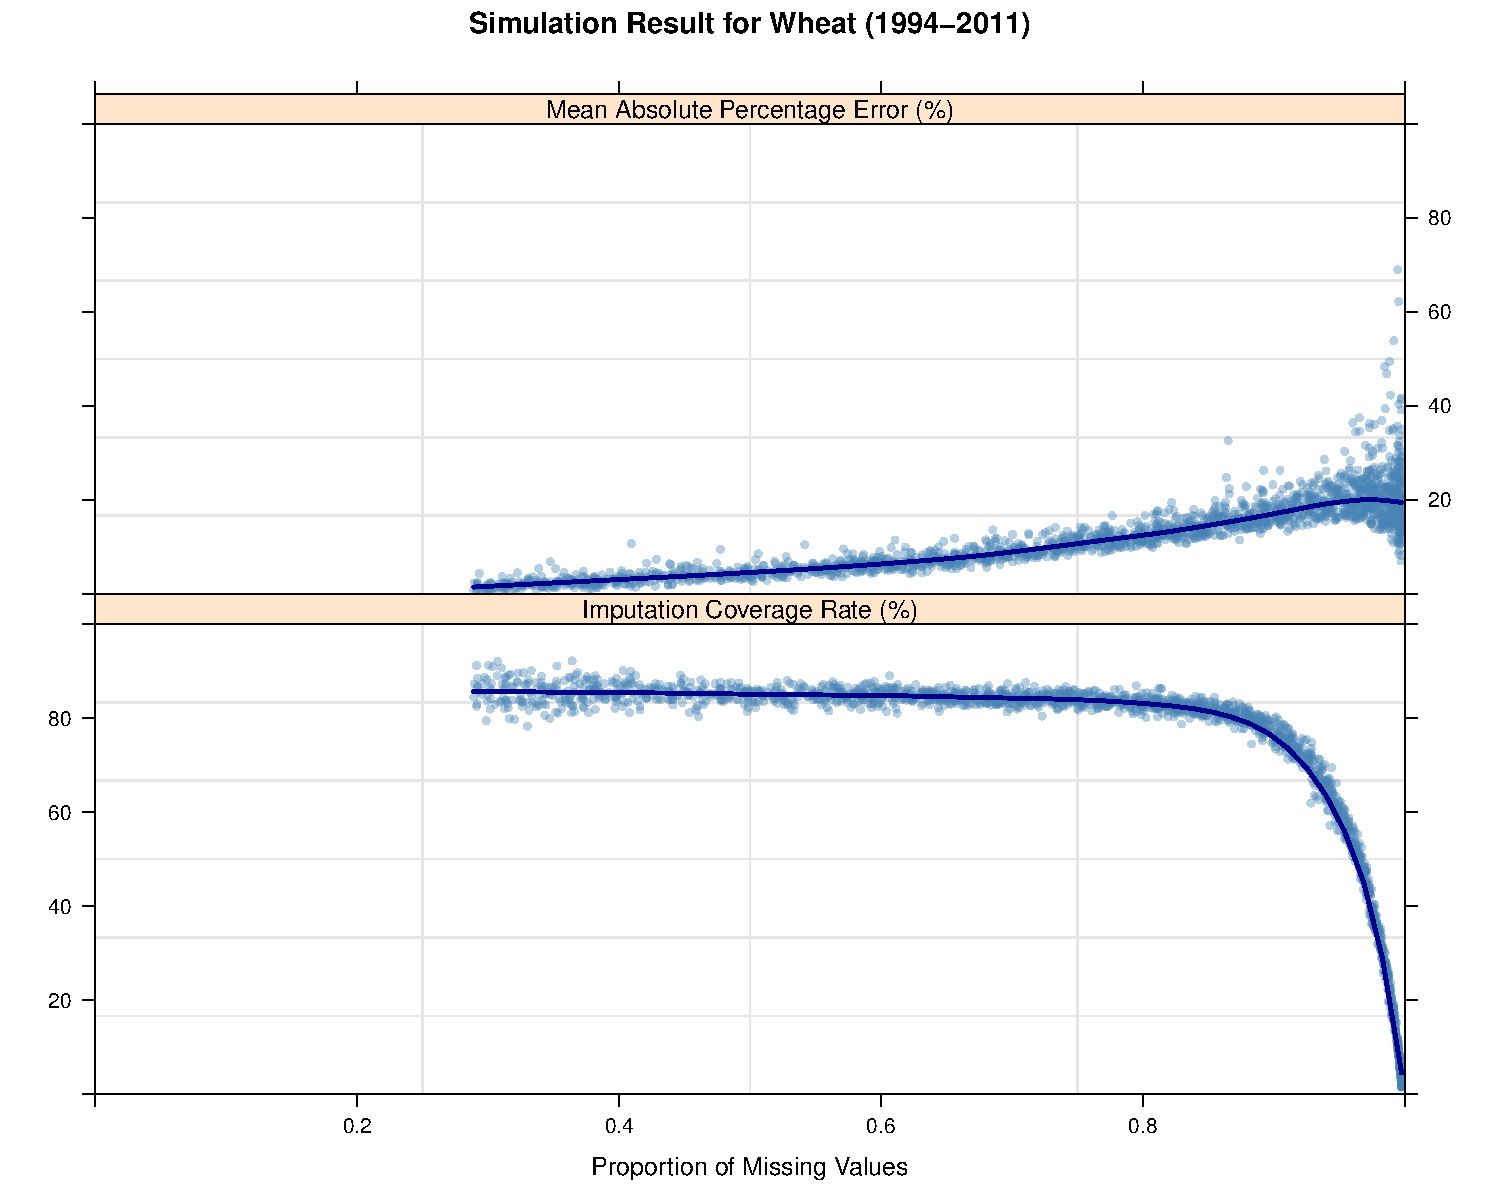
\includegraphics{wheatSimulationResult}
\end{figure}


\begin{figure}[ht!]
  \centering
  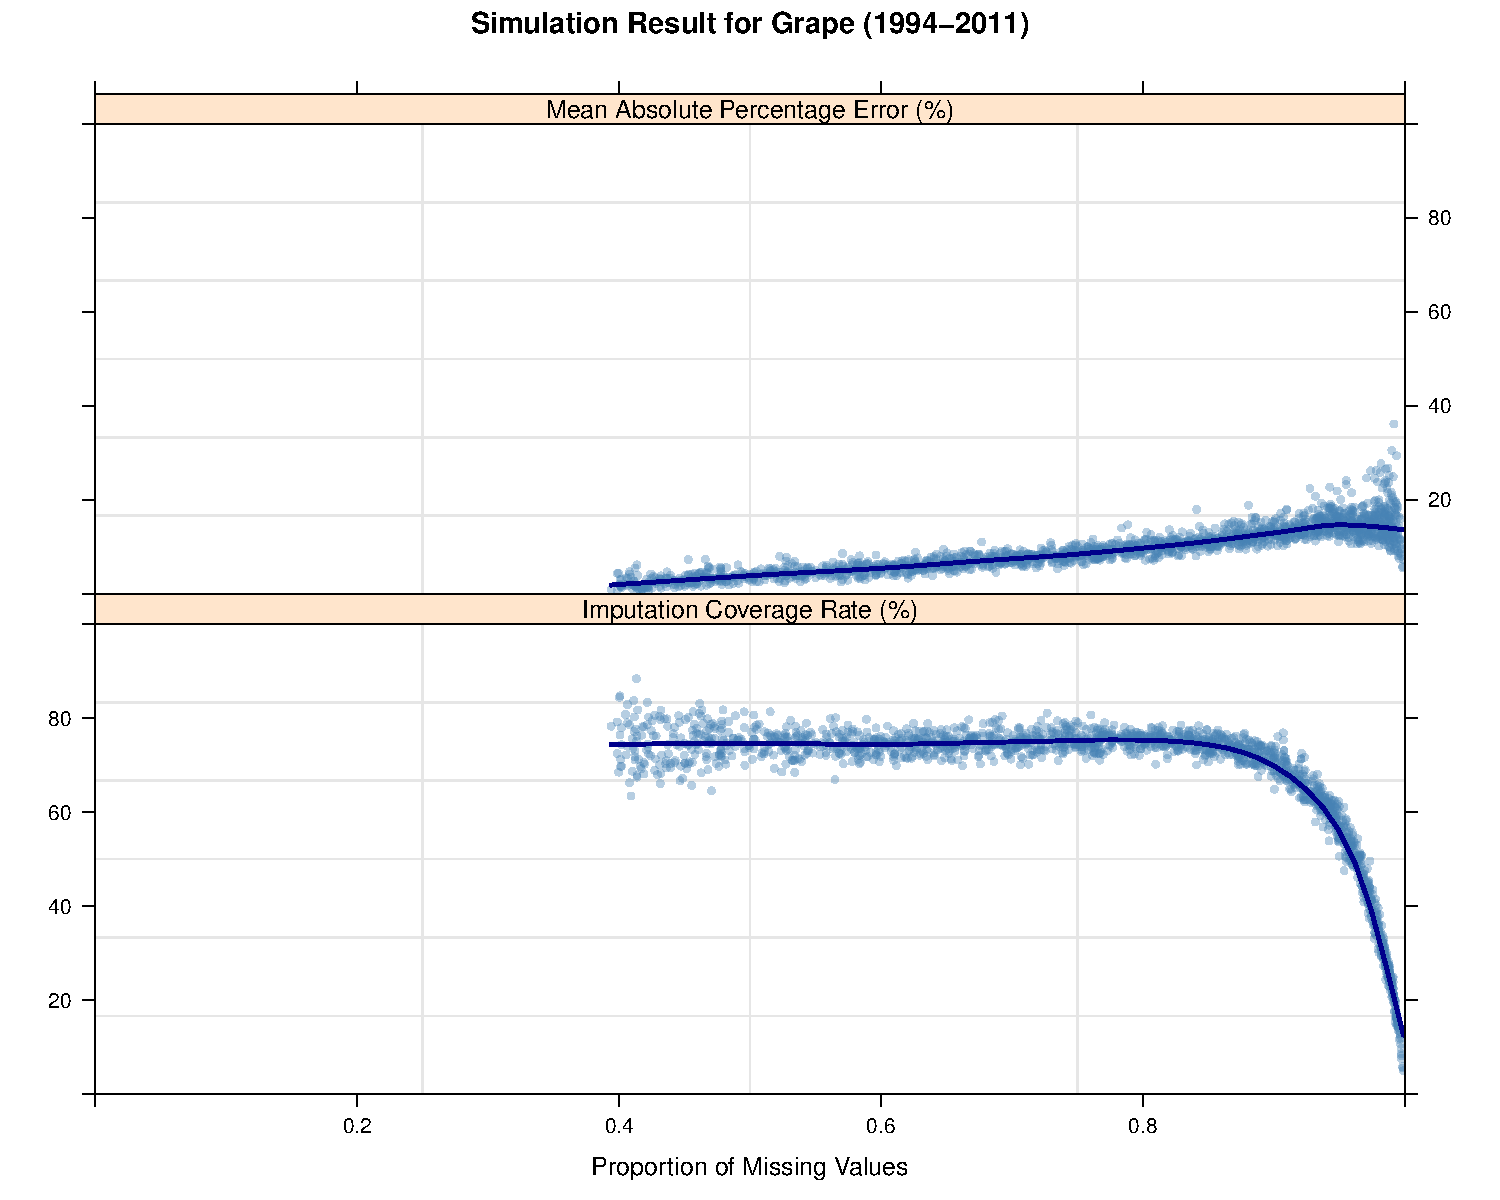
\includegraphics{grapeSimulationResult}
\end{figure}

\begin{figure}[ht!]
  \centering
  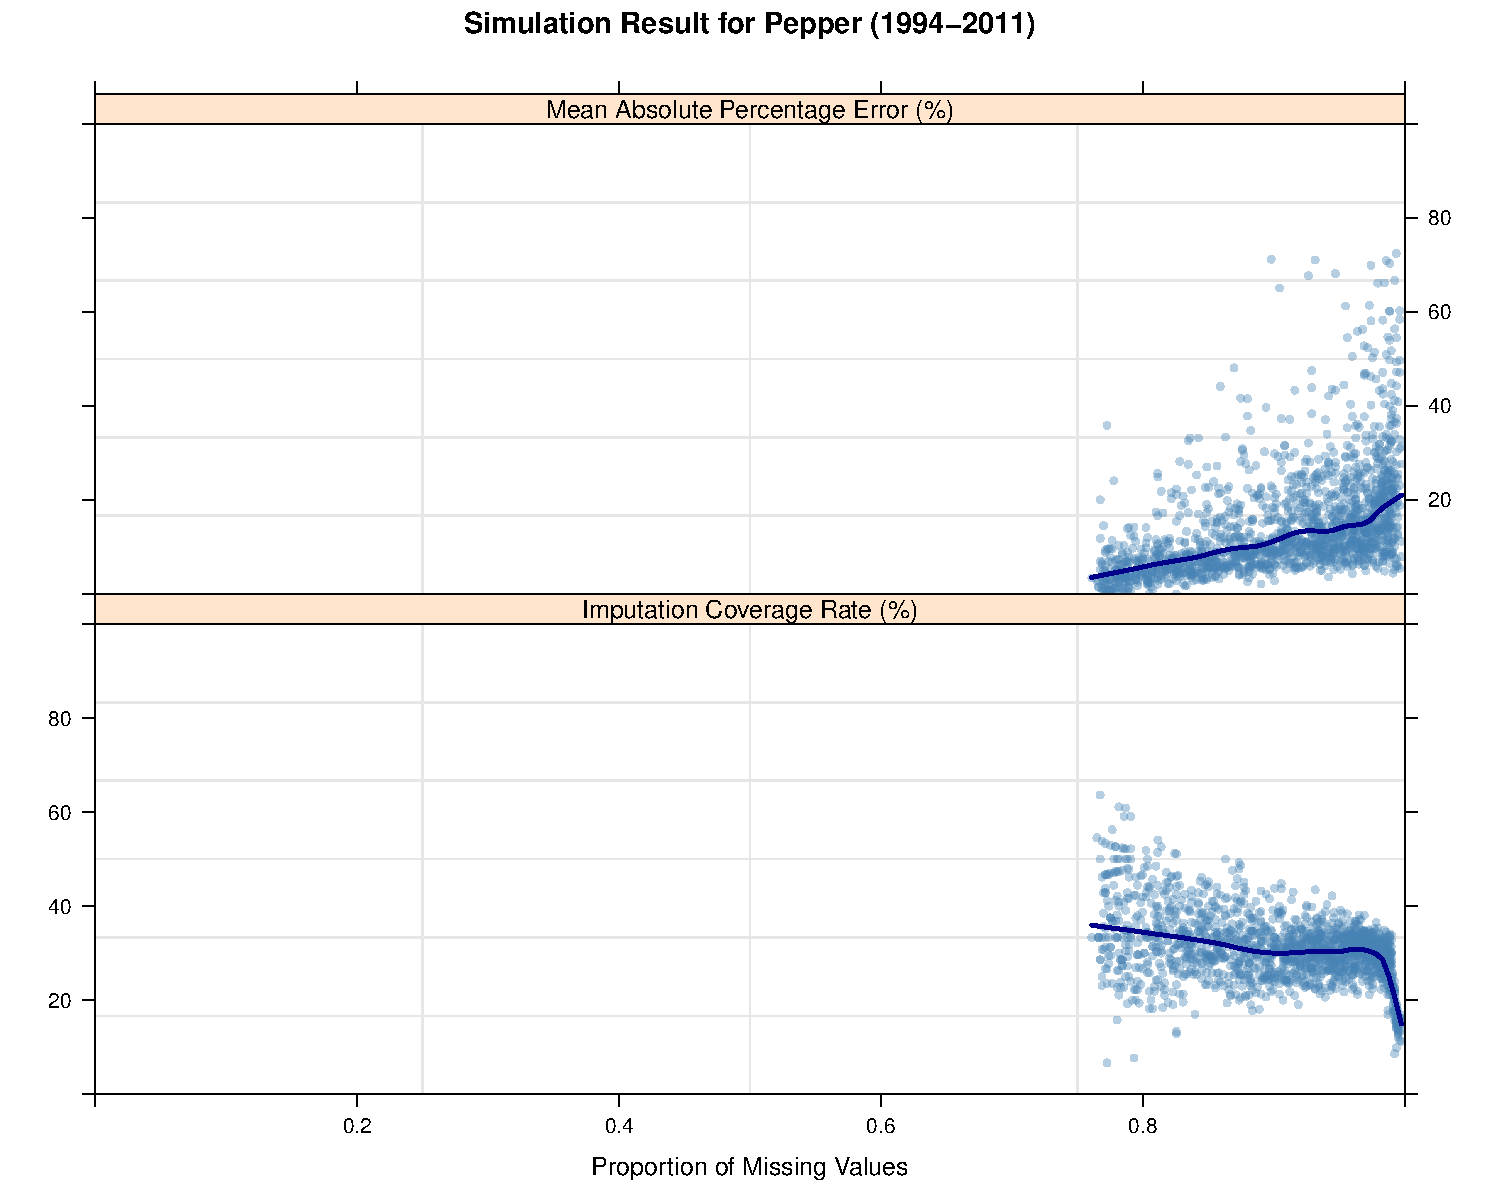
\includegraphics{pepperSimulationResult}
\end{figure}


\FloatBarrier
\section{Conclusion and Further Improvements}
The aim of the paper has been to overhaul the current imputation
methodology, with a more consistent, yet better performing approach.

The proposed model demonstrates the ability to resolve issues such as
diverging area and production series and biased growth as a result of
missing values. Furthermore, the proposal takes into account the
attribute of incorporating relevant information as well as
establishing a flexible framework to accommodate additional
information.

This is, however, work in progress, as the technical teams are
continuing to collaborate in order to seek a deeper understanding of
the data in order to improve on the model. Iterative imputation
methodology such as full conditional specification are considered to
imputed the area harvested, production and yield simultaneously.  In
addition, additive and robust mixed models are under-investigation for
country non-linearity departures and shocks.


\section*{Acknowledgement}
This work is supervised by Adam Prakash with assistance from Nicolas
Sakoff, Onno Hoffmeister, Luigi Castaldi, and Hansdeep Khaira whom
were crucial in the development of the methodology. The author would
also like to thank the team members which participated in the first
round of the discussion providing valuable feedbacks. Finally, credits
to Cecile Fanton and Frank Cachia whom devoted their time to translate
the paper into French.

\section*{Annex 1: Supplementary Resources}

The data, code implementation and documentation can all be found and
downloaded from \url{https://github.com/mkao006/sws_imputation}. This
paper is generated on \today and is subject to changes and updates.


\section*{Annex 2: Geographic and classification}

The geographic classification follows the UNSD M49 classification at
\url{http://unstats.un.org/unsd/methods/m49/m49regin.htm}. The
definition is also available in the \code{FAOregionProfile} of the R
package \pkg{FAOSTAT}.



\section*{Annex 3: Diagnostic graph of fit}

\begin{knitrout}
\definecolor{shadecolor}{rgb}{0.969, 0.969, 0.969}\color{fgcolor}\begin{figure}[!ht]


{\centering \includegraphics[width=\maxwidth]{figure/wheat-obs-fitted} 

}

\caption[Observed versus fitted value]{Observed versus fitted value\label{fig:wheat-obs-fitted}}
\end{figure}


\end{knitrout}



\begin{knitrout}
\definecolor{shadecolor}{rgb}{0.969, 0.969, 0.969}\color{fgcolor}\begin{figure}[!ht]


{\centering \includegraphics[width=\maxwidth]{figure/wheat-res-fitted} 

}

\caption[Residuals versus fitted value by country]{Residuals versus fitted value by country\label{fig:wheat-res-fitted}}
\end{figure}


\end{knitrout}


\begin{knitrout}
\definecolor{shadecolor}{rgb}{0.969, 0.969, 0.969}\color{fgcolor}\begin{figure}[!ht]


{\centering \includegraphics[width=\maxwidth]{figure/wheat-res-normality} 

}

\caption[Normality of residuals by country]{Normality of residuals by country\label{fig:wheat-res-normality}}
\end{figure}


\end{knitrout}



\begin{knitrout}
\definecolor{shadecolor}{rgb}{0.969, 0.969, 0.969}\color{fgcolor}\begin{figure}[!ht]


{\centering \includegraphics[width=\maxwidth]{figure/grape-obs-fitted} 

}

\caption[Observed versus fitted value]{Observed versus fitted value\label{fig:grape-obs-fitted}}
\end{figure}


\end{knitrout}



\begin{knitrout}
\definecolor{shadecolor}{rgb}{0.969, 0.969, 0.969}\color{fgcolor}\begin{figure}[!ht]


{\centering \includegraphics[width=\maxwidth]{figure/grape-res-fitted} 

}

\caption[Residuals versus fitted value by country]{Residuals versus fitted value by country\label{fig:grape-res-fitted}}
\end{figure}


\end{knitrout}


\begin{knitrout}
\definecolor{shadecolor}{rgb}{0.969, 0.969, 0.969}\color{fgcolor}\begin{figure}[!ht]


{\centering \includegraphics[width=\maxwidth]{figure/grape-res-normality} 

}

\caption[Normality of residuals by country]{Normality of residuals by country\label{fig:grape-res-normality}}
\end{figure}


\end{knitrout}


\FloatBarrier
\section*{Annex 4: Pseudo Codes}

\begin{algorithm}
  \SetAlgoLined
  \BlankLine
  Initialization\;
  \Indp\Indp\Indp 
  $\hat{Y}_{i, t} \leftarrow f(Y_{i, t})$\;
  $\cal{L}_{\text{old}} = -\infty$\;
  $\cal{E}$ = 1e-6\;
  n.iter = 1000\;
  \Indm\Indm\Indm

  %% (1) Estimate model without grouped average effect\;
  %% \Indp\Indp\Indp  
  %% $\hat{Y}_{i, t} \leftarrow \hat{\beta}_{0,j} + \hat{\beta}_{1,j}t +
  %% \hat{b}_{0i} + \hat{b}_{1i}t $\;
  %% \Indm\Indm\Indm
  
  %% (2) Estimate model with grouped average effect\;
  \Begin{
      \For{i=1 \emph{\KwTo} n.iter}{
        E-step: Compute the expected group average yield\;
        \Indp\Indp\Indp 
        $\mathbf{\hat{Y}^M} \leftarrow f(\mathbf{Y^O}, \boldsymbol{\hat{\beta}}^{(i)})$
        \Indm\Indm\Indm 
        
        M-step: Estimate the Linear Mix Model in \ref{eq:lmeImpute}\;
        \If{$\cal{L}_{\text{new}} - \cal{L}_{\text{old}} \ge
          \cal{E}$}{ $\boldsymbol{\hat{\beta}}^{(i + 1)} \leftarrow
          \boldsymbol{\hat{\beta}}$\; } \Else{ break } } }
    
    %% (3) Select model with the smallest AIC
    
    \caption{EM-Algorithm for Imputation}
    \label{alg:imputation}
\end{algorithm}
  
      

\begin{algorithm}[H]
  \SetAlgoLined
  \KwData{Production (element code = 51) and Harvested area (element
    code = 31) data}

  \KwResult{Imputation}
  
  \BlankLine
  Missing values are denoted $\emptyset$\;

  \BlankLine
  Initialization\;
  \Begin{
      \If{$A_t = 0 \land P_t \ne 0$}{
        $A_t \leftarrow \emptyset$\;
      }
      \If{$P_t = 0 \land A_t \ne 0$}{
        $P_t \leftarrow \emptyset$\;
      }
  }  
    
  \BlankLine  
  Start imputation\;
  \Begin{
      \ForAll{commodities}{
        
        (1) Compute the implied yield\;
        \Indp\Indp\Indp 
        $Y_{i,t} \leftarrow P_{i,t}/A_{i,t}$\;
        \Indm\Indm\Indm
                
        (2) Impute the missing yield with the imputation algorithm
        \ref{alg:imputation}\; \Indp\Indp\Indp
        
        \Indm\Indm\Indm        
        
        \ForAll{imputed yield $\hat{Y}_{i, t}$}{
          \If{$A_t = \emptyset \land P_t \ne \emptyset$}{
            $\hat{A}_{i, t} \leftarrow P_{i, t}/\hat{Y}_{i, t}$\;
          }
          \If{$P_t = \emptyset \land A_t \ne \emptyset$}{
            $\hat{P}_{i, t} \leftarrow A_{i, t} \times \hat{Y}_{i, t}$\;
          }
        }
        
        (4) Impute area ($A_{i, t}$) with equation
        \ref{eq:linearInterpolation} then \ref{eq:locf}\;
        
        \ForAll{imputed area $\hat{A}_{i, t}$}{ \If{$\hat{Y}_{i, t}
            \ne \emptyset$}{ $\hat{P}_{i, t} \leftarrow \hat{A}_{i, t}
            \times \hat{Y}_{i, t}$\; } } } }
  \caption{Imputation Procedure}
\end{algorithm}

  
  
\begin{thebibliography}{9}
\bibitem{dougbates2010}
  Douglas M. Bates
  \emph{lme4: Mixed-effects modelling with R}
  2010
  
\bibitem{impWorkingPaper2011}
  Data Collection, Workflows and Methodology (DCWM) team,
  \emph{Imputation and Validation Methodologies for the FAOSTAT Production Domain}.
  Economics and Social Statistics Division,
  2011.
  
\bibitem{lairdWare1982}
  Nan M. Laird, James H. Ware,
  \emph{Random-Effects Models for Longitudinal Data}.
  Biometrics Volume 38, 963-974,
  1982.
  
\bibitem{rCore}
  R Core Team,
  \emph{A language and environment for statistical computing.}
  R Foundation for Statistical Computing, Vienna, Austria.
  ISBN 3-900051-07-0, URL http://www.R-project.org/,
  2013.
  
\bibitem{nlme}
  Jose Pinheiro, Douglas Bates, Saikat DebRoy, Deepayan Sarkar and the
  R Development Core Team,
  \emph{nlme: Linear and Nonlinear Mixed Effects Models.} 
  R package version 3.1-108.
  2013

\bibitem{lme4}
  Douglas Bates, Martin Maechler, Ben Bolker and Steven Walker (2013).
  \emph{lme4: Linear mixed-effects models using Eigen and S4.} 
  R package version 1.0-4. http://CRAN.R-project.org/package=lme4
 
\bibitem{rubin1976}
  Donald B. Rubin,
  \emph{Inference and Missing Data},
  Biometrika, Volume 63, Issue 3, 581-592,
  1976
  
\bibitem{unido2012}
  Valentin Todorov, Matthias Templ
  \emph{R in the Statistical Office: Part II}
  2012
  
\bibitem{laird_ware1982}
  Nam M. Laird, James H. Ware
  \emph{Random-Effects Models for Longitudinal Data}
  Biometrics, Volume 38, Number 4, pp.963-974
  1982

\bibitem{dempster_laird_rubin1977}
  A. P. Dempster, Nam M. Laird, D. B. Rubin
  \emph{Maximum Likelihood from Incomplete Data via the EM Algorithm}
  Journal of Royal Statistical Society. Series B (Methodological), Volume 39, Number 1, pp1-38
  1977
  
\bibitem{lai_huang_lee2012}
  Randy C. S. Lai, Hsin-Cheng Huang, Thomase C. M. Lee
  \emph{Fixed and random effects selection in nonparametric additive mixed models}
  Electronic Journal of Statistics, Volume 6, pp810-842
  2012
\end{thebibliography}
  




\end{document}
